
% vim:set ff=unix expandtab ts=2 sw=2:
Since our poster template uses the beamer class,
we can influence the defaults for beamer blocks by the template.
(for example the background and foreground colors, fonts and font size for content and header of this box)
Which can help to avoid a lot of formatting in the user code and makes it easier to achieve a standard layout.
The interior is quite flexible.\\
\begin{itemize}
	\item we add a pseudo picture
\end{itemize}
	\begin{figure}[tb]
		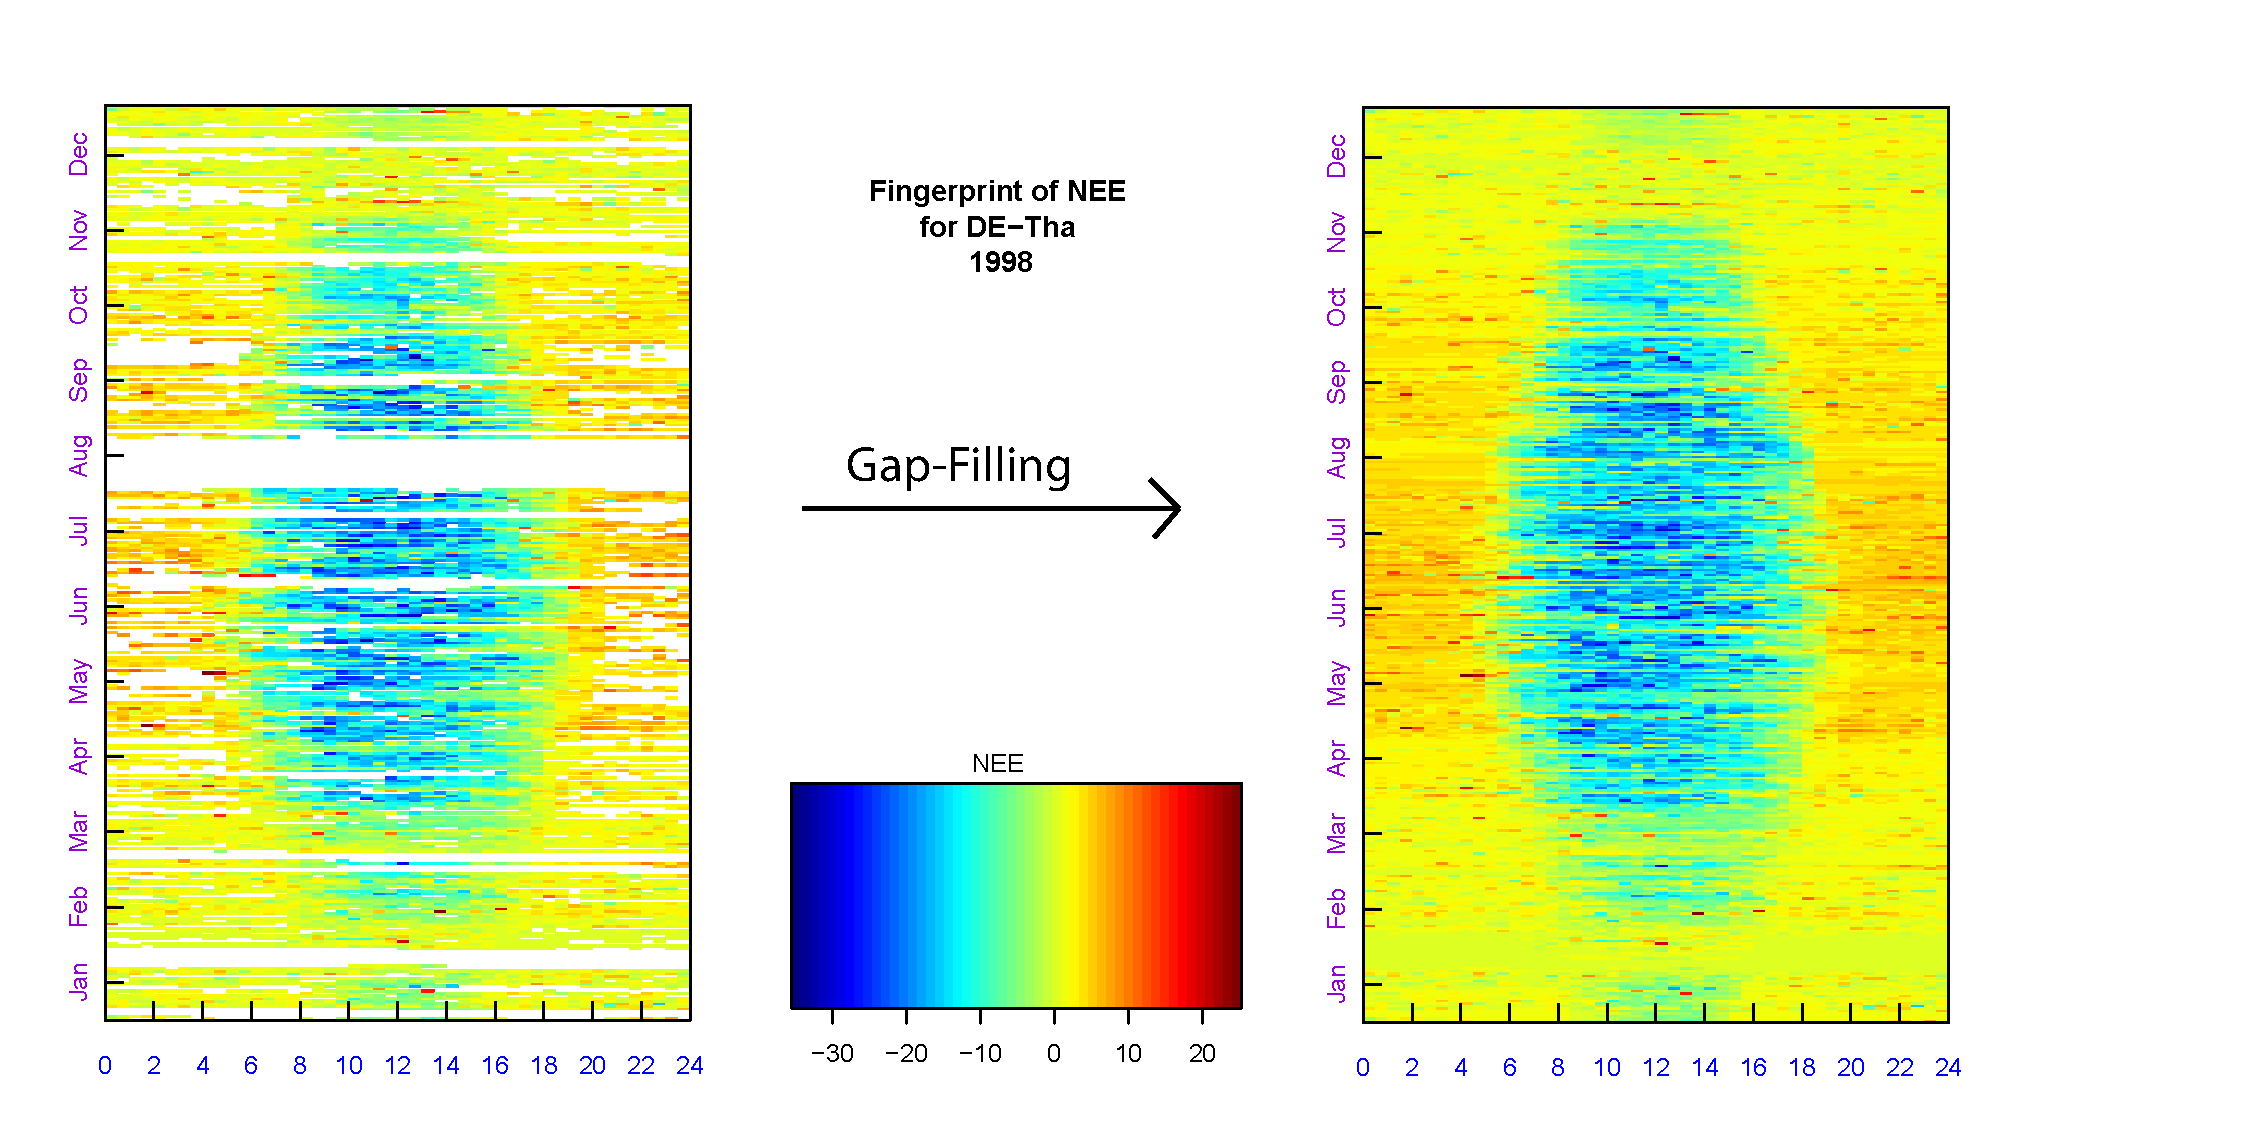
\includegraphics[height=3cm]{images/content/DE-Tha_1998_FP_NEE_ffc.pdf}
    \caption{a pseudo caption}
	\end{figure}



